\documentclass[12pt,a4paper]{article}
\usepackage[polish]{babel}
\usepackage[T1]{fontenc}
\usepackage{lmodern}
\usepackage[utf8x]{inputenc}
\usepackage{hyperref}
\usepackage{url}
\usepackage{graphicx}
\usepackage{listings}
%\usepackage{xcolor}
\usepackage{color}
\usepackage{float}
\usepackage{multicol}
\usepackage{tikz}

\usetikzlibrary{shapes.geometric, arrows}
\tikzstyle{startstop} = [rectangle, rounded corners, minimum width=3cm, minimum height=1cm,text centered, draw=black, fill=red!30]
\tikzstyle{io} = [trapezium, trapezium left angle=70, trapezium right angle=110, minimum width=3cm,text width=4cm, minimum height=1cm, text centered, draw=black, fill=blue!30]
\tikzstyle{process} = [rectangle, minimum width=3cm, minimum height=1cm, text centered, text width=4cm, draw=black, fill=orange!30]

\tikzstyle{decision} = [diamond, minimum width=3cm, minimum height=1cm, text centered, draw=black, fill=green!30]
\tikzstyle{arrow} = [thick,->,>=stealth]

\addtolength{\hoffset}{-1.5cm}
\addtolength{\marginparwidth}{-1.5cm}
\addtolength{\textwidth}{3cm}
\addtolength{\voffset}{-1cm}
\addtolength{\textheight}{2.5cm}
\setlength{\topmargin}{0cm}
\setlength{\headheight}{0cm}

%\lstset{
%    numbers=left,
%    breaklines=true,
%    tabsize=2,
%    basicstyle=\ttfamily,
%    frame=lr,
%    rulecolor=\color{blue!80!black},
%    language=[Sharp]C
%}
\definecolor{bluekeywords}{rgb}{0,0,1}
\definecolor{greencomments}{rgb}{0,0.5,0}
\definecolor{redstrings}{rgb}{0.64,0.08,0.08}
\definecolor{xmlcomments}{rgb}{0.5,0.5,0.5}
\definecolor{types}{rgb}{0.17,0.57,0.68}
\lstset{language=[Sharp]C,
captionpos=b,
frame=lines,
showspaces=false,
showtabs=false,
breaklines=true,
showstringspaces=false,
breakatwhitespace=true,
escapeinside={(*@}{@*)},
commentstyle=\color{greencomments},
morekeywords={partial, var, value, get, set},
keywordstyle=\color{bluekeywords},
stringstyle=\color{redstrings},
basicstyle=\ttfamily\small,
tabsize=4,
}

\begin{document}
	
	\title{Systemy Sztucznej Inteligencji\\\small{Dokumentacja projektu Unity Neural Network Car}}
	\author{Artur Bednarczyk, Dawid Grajewski, grupa A}
	\date{\today}

	\maketitle
	\newpage
	\tableofcontents
	\newpage
	\section{Część I}
	\subsection{Opis programu}
	Unity Neural Network Car to symulacja samochodu poruszającego się po torze. Jednak nie tylko użytkownik może kontrolować pojazd, a również sztuczna inteligencja. Implementacja zaawansowanej technologii pozwoliła na ,,nauczenie'' samochodu w jaki sposób przejechać przez cały tor i nie rozbić się na najbliższym zakręcie.
	\begin{figure}[H]
	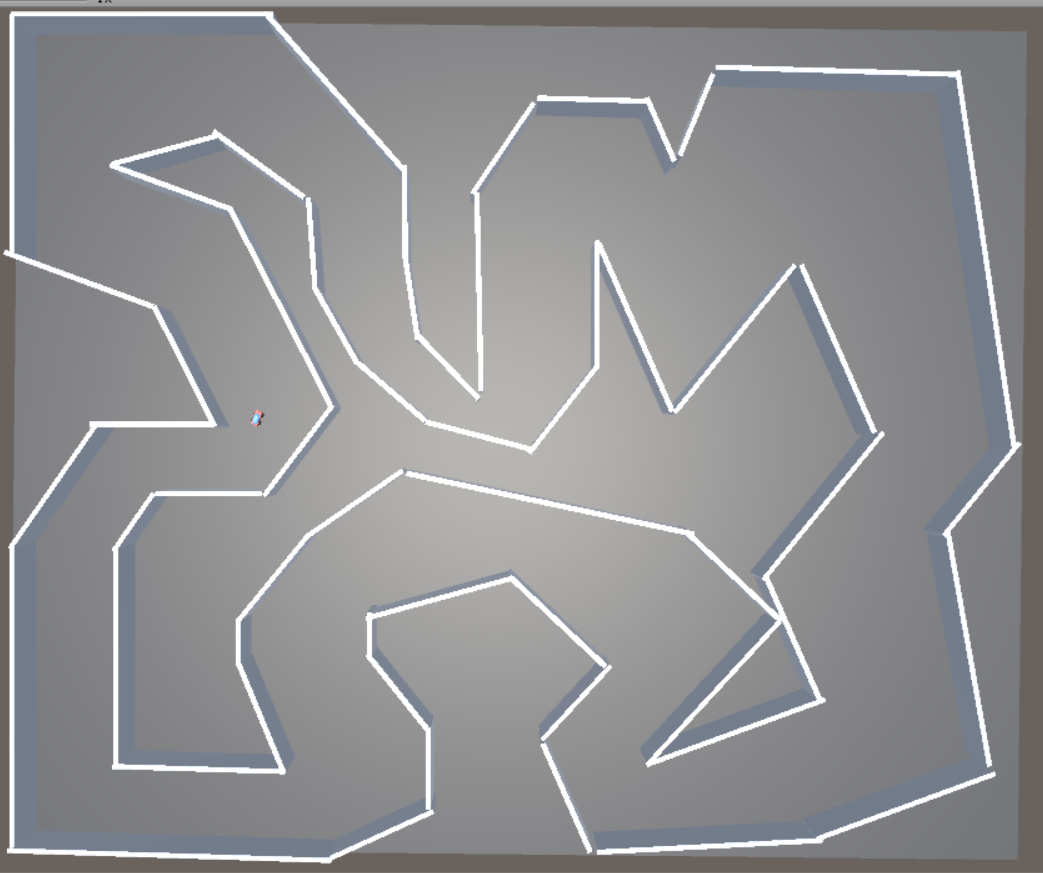
\includegraphics[scale=0.7]{car}
	\centering
	\end{figure}
	\subsection{Instrukcja obsługi}
	Uruchamiamy aplikację i możemy obserwować ruch pojazdu.
	\subsection{Dodatkowe informacje}
	Projekt został wykonany z wykorzystaniem silnika Unity oraz języka C\#.
	\newpage
	\section{Część II}
	\subsection{Opis działania} 
\subsubsection{Sieć neuronowa}
Sieć neuronowa jest strukturą inspirowaną budową naturalnych neuronów, łączących je synaps oraz układów nerwowych. Wykorzystana w projekcie sieć jest wielowarstwową siecią jednokierunkową korzystającą z algorytmu propagacji wstecznej.
\subsubsection{Budowa sieci}
Wykorzystana sieć składa się z trzech głównych warstw.
\begin{itemize}
	\item Warstwa wejścia.
	\item Warstwy ukryte.
	\item Warstwa wyjścia.
\end{itemize}
\paragraph*{Warstwa wejścia} Każdy neuron tej warstwy przekazuje do warstwy ukrytej początkowe wartości.
\paragraph*{Warstwy ukryte} Tutaj dzieje się wszystko co najważniejsze. Synapsy między neuronami mają przypisane wagi, które początkowo są losowe. W ramach uczenia się, wagi są dostosowywane tak, aby rezultat końcowy był jak najbliżej spodziewanego.
\paragraph*{Warstwa wyjścia} To tutaj nauczona już sieć daje nam wynik.
\subsubsection{Uczenie sieci}
Uczenie sieci jest realizowane poprzez podanie jej zestawu danych wejściowych oraz spodziewanych wyników. W tym projekcie wykorzystano metody takie jak:
\begin{itemize}
\item Propagacja Wsteczna
\item Biases
\item Momentum
\item Współczynnik uczenia
\end{itemize}

\paragraph*{Propagacja wsteczna} to podstawowy algorytm uczenia nadzorowanego wielowarstwowych, jednokierunkowych sieci neuronowych. Dzięki wstecznej propagacji błędu możemy dobrać odpowiednie wagi we wszystkich warstwach sieci. Początkowo dla losowych wag obliczane są błędy, czyli różnica między odpowiedzią obliczoną a spodziewaną, które następnie są propagowane do wcześniejszych warstw. Wagi zostają modyfikowane na podstawie błędu i obliczonych danych. Algorytm jest zostaje zatrzymany, gdy średnia wartość błędu przestanie maleć.
\paragraph*{Biases} Są to wartości, które pozwalają na przesunięcie funkcji aktywacji w sposób, na który zmiana wagi nie pozwala. Przykład funkcji bez bias:
\begin{figure}[H]
\centering
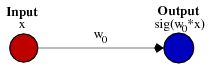
\includegraphics[scale=0.7]{biases_01}
\caption{https://stackoverflow.com/questions/2480650/role-of-bias-in-neural-networks}
\end{figure}
\begin{figure}[H]
\centering
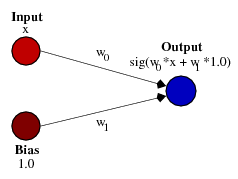
\includegraphics[scale=0.5]{biases_03}
\caption{https://stackoverflow.com/questions/2480650/role-of-bias-in-neural-networks}
\end{figure}\clearpage
Przykład funkcji z bias:
\begin{figure}[H]
\centering
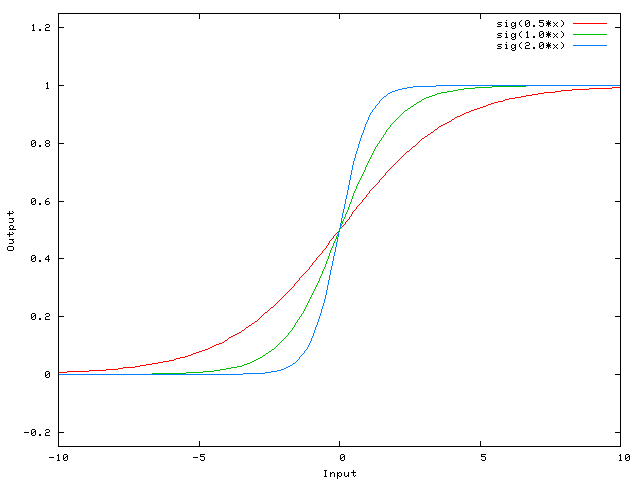
\includegraphics[scale=0.7]{biases_02}
\caption{https://stackoverflow.com/questions/2480650/role-of-bias-in-neural-networks}
\end{figure}
\begin{figure}[H]
\centering
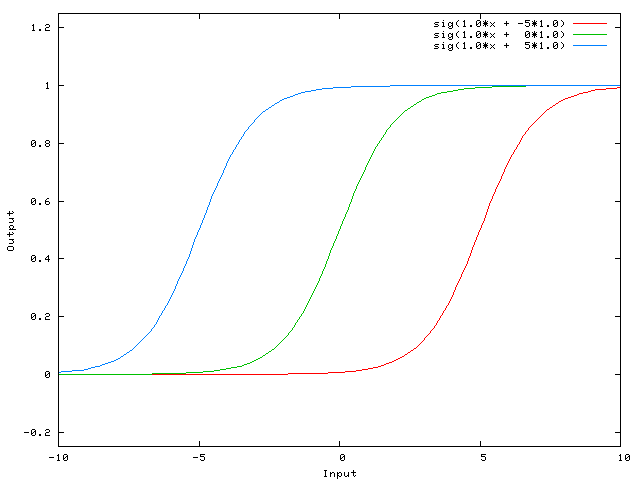
\includegraphics[scale=0.5]{biases_04}
\caption{https://stackoverflow.com/questions/2480650/role-of-bias-in-neural-networks}
\end{figure}
Wykorzystanie tego jest konieczne aby uczenie zostało zrealizowane z prawidłowymi wynikami.
\paragraph*{Momentum} Jest to współczynnik odpowiadający za dodanie ułamka poprzedniej wagi do aktualnej. Używany jest aby zapobiec zbieżności do lokalnego minimum lub punktu siodłowego. Wysoka wartość tego współczynnika przyspiesza proces konwergencji, jednakże zbyt wysoka może spowodować, że cały system stanie się niestabilny, a zbyt niska spowolni proces uczenia.
\paragraph*{Współczynnik uczenia} to współczynnik odpowiadający za to jak duże są zmiany wag oraz biasów.
\subsubsection{Funkcja Aktywacji}
Wartość wyjścia neuronów jest obliczana za pomocą funkcji aktywacji. W tym projekcie została użyta funkcja sigmoidalna:
$$ S(x) = \frac{1}{1+e^{-x}} = \frac{e^x}{e^x+1} $$
\begin{figure}[H]
\centering
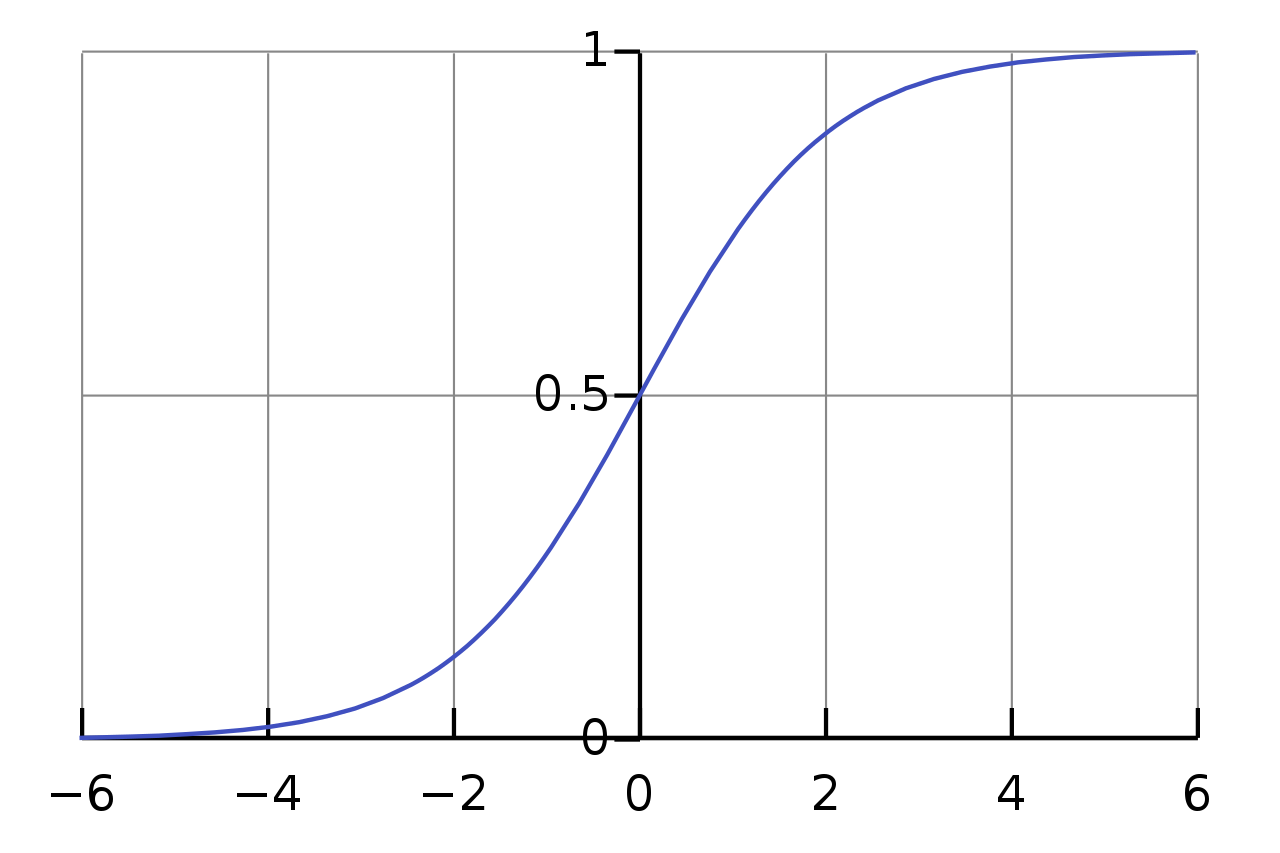
\includegraphics[scale=0.5]{sigmoid}
\caption{https://en.wikipedia.org/wiki/Sigmoid\_function}
\end{figure}
Funkcja ta przyjmuje wartości od 0 do 1.
	\subsection{Algorytm}
	\begin{figure}[H]
		\centering

	\begin{tikzpicture}[node distance=2cm]
		\node (start) [startstop] {START};
		\node (dec1) [decision, below of=start, yshift=-1.0cm]{Jeśli sieć nauczona.};
		\node (in1) [io, left of=dec1, xshift=-4.3cm]{Pobranie danych treningowych};
		\node (pro1) [process, below of=in1]{Uczenie sieci};
		\node (out1) [io, below of=pro1]{Zapis danych};
		\node (pro2) [process, below of=out1] {Podłączenie sieci do auta};
		\node (pro3) [process, below of=pro2] {Auto jedzie.} ;
		\node (stop) [startstop, below of=pro3] {STOP};
		
		
		\draw [arrow](start) -- node {}(dec1);
		\draw [arrow] (dec1) -- node[anchor=south] {Nie} (in1);
		\draw [arrow] (dec1) |- node[anchor=west] {Tak} (pro2);
		\draw [arrow] (in1) -- node {} (pro1);
		\draw [arrow] (pro1) -- node {} (out1);
		\draw [arrow] (out1) -- node {} (pro2);
		\draw [arrow] (pro2) -- node {} (pro3);
		\draw [arrow] (pro3) -- node {} (stop);
	\end{tikzpicture}	\end{figure}\clearpage
	
	\subsection{Bazy danych}
	Zestaw danych wykorzystany do uczenia sieci:
	\begin{multicols}{3}
	\begin{verbatim}
	14.85;14.85;0
15.2;14.53;-0.58
13.32;17.02;1
14.13;15.67;0.91
15.17;14.55;-0.55
11.15;17.01;1
11.61;13.86;0.98
12;12.78;0.65
12.11;12.54;0.41
12.27;12.21;-0.06
9.19;10.16;0.75
11.7;11.57;-0.13
21.19;30.54;1
11.52;13.08;0.92
15.13;14.7;-0.41
13.91;5.75;-1
27.65;7.57;-1
25.97;28.01;0.97
2.45;34.22;1
6.81;25.24;1
16.07;9.18;-1
8.77;28.54;1
53.54;16.19;-1
14.85;14.85;0
11.91;20.92;1
15.48;13.44;-0.97
11.55;42.66;1
9.13;57.46;1
11.39;8.89;-0.99
8.77;17.61;1
6.76;11.94;1
9.29;17.88;1
11.99;14.92;0.99
14.62;23.18;1
9.26;43.26;1
11.42;11.28;-0.14
27.01;15.2;-1
46.28;12.89;-1
9.78;42.4;1
9.7;34.88;1
16.85;29.69;1
13.93;32.74;1
11.93;22.02;1
11.85;12.9;0.78
11.65;13.09;0.89
11.47;13.27;0.95
11.28;36.85;1
16.38;59.26;1
13.28;17.18;1
21.74;9.69;-1
14.12;15.83;0.94
8.96;46.62;1
10.84;25.92;1
10.43;14.23;1
11.96;12.46;0.46
8.41;56.14;1
9.51;9.86;0.34
9.58;9.8;0.22
8.58;34.3;1
11.4;28.29;1
12.04;18.61;1
9.9;12.58;0.99
11.4;12.29;0.71
21.91;14.5;-1
27.92;10.77;-1
10.56;41.72;1
12.83;34.31;1
22.76;12.84;-1
14.72;41.8;1
10.84;17.78;1
13.08;11.69;-0.88
11.38;13.75;0.98
12.49;44.46;1
18.94;62.05;1
14.82;15.15;0.32
15.99;13.69;-0.98
14.75;14.95;0.2
14.61;15.09;0.45
13.22;25.17;1
8.73;44.85;1
12.02;13.28;0.85
8.11;18.57;1
9.59;9.82;0.23
8;11.66;1
9.77;32.76;1
12.85;12.84;-0.01
17.03;20.62;1
10.1;13.55;1
29.72;11.01;-1
23.51;24.2;0.6
10.39;14.55;1
9.35;38.1;1
14.44;31.04;1
17.75;45.91;1
15.47;8.69;-1
10.89;21.47;1
11.22;13.82;0.99
11.57;13.18;0.92
13.29;40.47;1
16.3;27.81;1
14.79;14.91;0.12
14.79;14.91;0.12
17.33;13.24;-1
14.83;14.86;0.03
14.83;14.86;0.03
15.97;13.94;-0.97
15.97;13.94;-0.97
14.82;14.87;0.05
13.13;17.46;1
14.07;15.7;0.93
13.51;16.47;0.99
14.15;15.53;0.88
12.79;17.21;1
12.02;48.39;1
10.48;16.74;1
10.48;16.74;1
11.78;12.9;0.81
11.78;12.9;0.81
14.1;10.7;-1
14.1;10.7;-1
12.61;11.8;-0.67
12.61;11.8;-0.67
12.6;11.81;-0.66
10.3;53.25;1
9.32;56.21;1
11.54;7.91;-1
10.98;8.66;-0.98
17.35;6.73;-1

	\end{verbatim}
	\end{multicols}
	\subsection{Implementacja}
	Projekt powstał z wykorzystaniem narzędzi Unity. Funkcjonalność została zawarta w folderze Assets/Scripts, którego zawartość wygląda następująco:
	\begin{itemize}
	\item Controllers 
		\begin{itemize}
		\item AutonomicCarController.cs
		\item BrainController.cs
		\item CarController.cs
		\item ManualCarController.cs
		\end{itemize}
	\item NeuralNetwork
		\begin{itemize}
		\item Helpers
			\begin{itemize}
			\item ExportHelper.cs
			\item HelperNetwork.cs
			\item ImportHelper.cs
			\end{itemize}
		\item NetworkModels
			\begin{itemize}
			\item Dataset.cs
			\item Network.cs
			\item Neuron.cs
			\item Sigmoid.cs
			\item Synapse.cs
			\end{itemize}
		\end{itemize}
	\item Serializers
		\begin{itemize}
		\item ISerializer.cs
		\item XmlSerializer.cs
		\end{itemize}
	\end{itemize}
	
	Klasy i opis ich metod:
	\begin{itemize}
		\item AutonomicCarController.cs
			\begin{itemize}
				\item Update() - Wywołuje metodę sprawdzającą dystans do ścian, metodę ruchu i metodę sterowania.
			\end{itemize}
		\item BrainController.cs
			\begin{itemize}
				\item Compute(double,double) - Pobiera z sieci wynik na podstawie odległości od ścian.
				\item Load() - Odtworzenie sieci neuronowej z wskazanego pliku.
				\item Save() - Zapis instancji sieci neuronowej do wskazanego pliku.
				\item TestNetwork() - Testuje sieć.
				\item Train() - Uczy sieć na podstawie danych z wskazanego pliku.
			\end{itemize}
		\item CarController.cs
			\begin{itemize}
				\item MoveForward() - Ruch do przodu.
				\item TurnLeft() - Skręt w lewo.
				\item TurnRight() - Skręt w prawo.
				\item Update() - Wywołuje metodę sprawdzającą dystans do ścian.
			\end{itemize}
		\item ManualCarController.cs
			\begin{itemize}
				\item Update() - Wywołuje metodę sprawdzającą dystans do ścian oraz jeśli zbiera dane to wywołuje metodę zbierającą dane do uczenia.
			\end{itemize}
		\item ExportHelper.cs
			\begin{itemize}
				\item ExportNetwork(Network, string, ISerializer) - wywołuje metodę pobierającą sieć i eksportuje są do pliku.
			\end{itemize}
		\item HelperNetwork.cs
			\begin{itemize}
				\item HelperNetwork() - Konstruktor tworzący listy neuronów dla warstwy wejściowej, wyjściowej, listę list neuronów warstw ukrytych oraz listę synaps.
			\end{itemize}
		\item ImportHelper.cs
			\begin{itemize}
				\item ImportNetwork(string, ISerializer) - Importuje sieć z pliku.
			\end{itemize}
		\item Dataset.cs
			\begin{itemize}
				\item DataSet(double[], double[]) - Konstruktor klasy DataSet.
			\end{itemize}
		\item Network.cs
			\begin{itemize}
				\item Compute(double[]) - Wywołuje metodę przedniej propagacji i pobiera wyniki z warstwy wyjściowej.
				\item GetRandom() - Zwraca losową liczbę.
				\item Network() - Konstruktor.
				\item Network(int,int[],int,double?,double?,bool) - Konstruktor.
				\item Train(List<DataSet>,double) - Wywołuje metody propagacji aż średni błąd będzie mniejszy niż podano.
				\item Train(List<DataSet>,int) - Wywołuje metody propagacji aż zostanie osiągnięta określona liczba powtórzeń.
			\end{itemize}
		\item Neuron.cs
			\begin{itemize}
				\item CalculateError(double) - Oblicza błąd
				\item CalculateGradient(double?) - Oblicza gradient.
				\item CalculateValue() - Oblicza wartość.
				\item Neuron() - Konstruktor.
				\item Neuron(IEnumerable<Neuron>) - Tworzy połączenia synaps między neuronami.
				\item UpdateWeights(double,double) - Aktualizuje wagi.
			\end{itemize}
		\item Sigmoid.cs
			\begin{itemize}
				\item Output(double) - Zwraca wynik funkcji w zależności od podanej wartości.
				\item Derivative(double) - zwraca pochodną funkcji.
			\end{itemize}
		\item Synapse.cs
			\begin{itemize}
				\item Synapse() - Konstruktor.
				\item Synapse(Neuron,Neuron) - Konstruktor z wejściowym i wyjściowym neuronem.
			\end{itemize}
		\item XmlSerializer.cs
			\begin{itemize}
				\item Deserialize(string) - Odczytuje sieć z pliku.
				\item Serialize(HelperNetwork, string) - Zapisuje sieć do pliku.
			\end{itemize}
	\end{itemize}

	\subsection{Testy}
	Sieć działa prawidłowo. Samochód porusza się po torze w sposób zadowalający.	\\
	\paragraph{Wykres błędów}:\\
	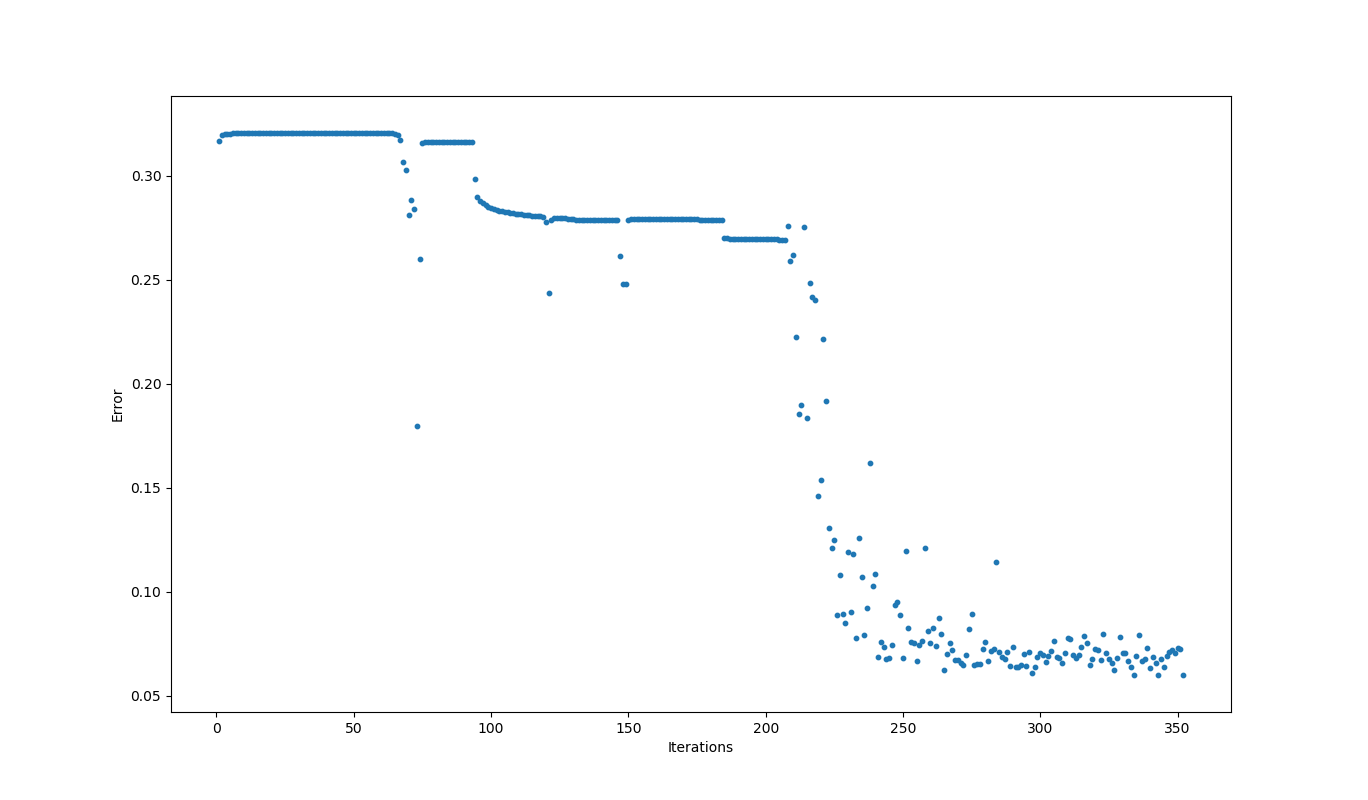
\includegraphics[scale=0.5]{supa_wykres}
	\newpage
	\section{Pełen kod aplikacji}
	\subsection{Neuron}
	\begin{lstlisting}
public class Neuron
{
	#region -- Properties --
	public Guid Id { get; set; }
	public List<Synapse> InputSynapses { get; set; }
	public List<Synapse> OutputSynapses { get; set; }
	public double Bias { get; set; }
	public double BiasDelta { get; set; }
	public double Gradient { get; set; }
	public double Value { get; set; }
	#endregion

	#region -- Constructors --
	public Neuron()
	{
		Id = Guid.NewGuid();
		InputSynapses = new List<Synapse>();
		OutputSynapses = new List<Synapse>();
		Bias = Network.GetRandom();
	}

	public Neuron(IEnumerable<Neuron> inputNeurons) : this()
	{
		foreach (var inputNeuron in inputNeurons)
		{
			var synapse = new Synapse(inputNeuron, this);
			inputNeuron.OutputSynapses.Add(synapse);
			InputSynapses.Add(synapse);
		}
	}
	#endregion

	#region -- Values & Weights --
	public virtual double CalculateValue()
	{
		return Value = Sigmoid.Output(InputSynapses.Sum(a => a.Weight * a.InputNeuron.Value) + Bias);
	}

	public double CalculateError(double target)
	{
		return target - Value;
	}

	public double CalculateGradient(double? target = null)
	{
		if (target == null)
			return Gradient = OutputSynapses.Sum(a => a.OutputNeuron.Gradient * a.Weight) * Sigmoid.Derivative(Value);

		return Gradient = CalculateError(target.Value) * Sigmoid.Derivative(Value);
	}

	public void UpdateWeights(double learnRate, double momentum)
	{
		var prevDelta = BiasDelta;
		BiasDelta = learnRate * Gradient;
		Bias += BiasDelta + momentum * prevDelta;

		foreach (var synapse in InputSynapses)
		{
			prevDelta = synapse.WeightDelta;
			synapse.WeightDelta = learnRate * Gradient * synapse.InputNeuron.Value;
			synapse.Weight += synapse.WeightDelta + momentum * prevDelta;
		}
	}
	#endregion
}
	\end{lstlisting}
	\clearpage
	\subsection{Synapse}
	\begin{lstlisting}
	public class Synapse
	{
		#region -- Properties --
		public Guid Id { get; set; }
		public Neuron InputNeuron { get; set; }
		public Neuron OutputNeuron { get; set; }
		public double Weight { get; set; }
		public double WeightDelta { get; set; }
		#endregion

		#region -- Constructor --
		public Synapse() { }

		public Synapse(Neuron inputNeuron, Neuron outputNeuron)
		{
			Id = Guid.NewGuid();
			InputNeuron = inputNeuron;
			OutputNeuron = outputNeuron;
			Weight = Network.GetRandom();
		}
		#endregion
	}
	\end{lstlisting}
	
	\subsection{Network}
	\begin{lstlisting}
	public class Network
	{
		#region -- Properties --
		public double LearnRate { get; set; }
		public double Momentum { get; set; }
		public List<Neuron> InputLayer { get; set; }
		public List<List<Neuron>> HiddenLayers { get; set; }
		public List<Neuron> OutputLayer { get; set; }
        public bool ShowIterationError { get; set; }
		#endregion

		#region -- Globals --
		private static readonly Random Random = new Random();
		#endregion

		#region -- Constructor --
		public Network()
		{
			LearnRate = 0;
			Momentum = 0;
			InputLayer = new List<Neuron>();
			HiddenLayers = new List<List<Neuron>>();
			OutputLayer = new List<Neuron>();
		}

        public Network(int inputSize, int[] hiddenSizes, int outputSize, double? learnRate = null, double? momentum = null, bool showIterationError = false)
		{
            ShowIterationError = showIterationError;
			LearnRate = learnRate ?? .4;
			Momentum = momentum ?? .9;
			InputLayer = new List<Neuron>();
			HiddenLayers = new List<List<Neuron>>();
			OutputLayer = new List<Neuron>();

			for (var i = 0; i < inputSize; i++)
				InputLayer.Add(new Neuron());

			var firstHiddenLayer = new List<Neuron>();
			for (var i = 0; i < hiddenSizes[0]; i++)
				firstHiddenLayer.Add(new Neuron(InputLayer));

			HiddenLayers.Add(firstHiddenLayer);

			for (var i = 1; i < hiddenSizes.Length; i++)
			{
				var hiddenLayer = new List<Neuron>();
				for (var j = 0; j < hiddenSizes[i]; j++)
					hiddenLayer.Add(new Neuron(HiddenLayers[i - 1]));
				HiddenLayers.Add(hiddenLayer);
			}

			for (var i = 0; i < outputSize; i++)
				OutputLayer.Add(new Neuron(HiddenLayers.Last()));
		}
		#endregion

		#region -- Training --
		public void Train(List<DataSet> dataSets, int numEpochs)
		{
			for (var i = 0; i < numEpochs; i++)
			{
				foreach (var dataSet in dataSets)
				{
					ForwardPropagate(dataSet.Values);
					BackPropagate(dataSet.Targets);
				}
			}
		}

		public void Train(List<DataSet> dataSets, double minimumError)
		{
			var error = 1.0;
			var numEpochs = 0;

			while (error > minimumError && numEpochs < int.MaxValue)
			{
				var errors = new List<double>();
				foreach (var dataSet in dataSets)
				{
					ForwardPropagate(dataSet.Values);
					BackPropagate(dataSet.Targets);
					errors.Add(CalculateError(dataSet.Targets));
				}
				error = errors.Average();
                numEpochs++;

                if(ShowIterationError)
                    Console.WriteLine(error);
			}
		}

		private void ForwardPropagate(params double[] inputs)
		{
			var i = 0;
			InputLayer.ForEach(a => a.Value = inputs[i++]);
			HiddenLayers.ForEach(a => a.ForEach(b => b.CalculateValue()));
			OutputLayer.ForEach(a => a.CalculateValue());
		}

		private void BackPropagate(params double[] targets)
		{
			var i = 0;
			OutputLayer.ForEach(a => a.CalculateGradient(targets[i++]));
			HiddenLayers.Reverse();
			HiddenLayers.ForEach(a => a.ForEach(b => b.CalculateGradient()));
			HiddenLayers.ForEach(a => a.ForEach(b => b.UpdateWeights(LearnRate, Momentum)));
			HiddenLayers.Reverse();
			OutputLayer.ForEach(a => a.UpdateWeights(LearnRate, Momentum));
		}

		public double[] Compute(params double[] inputs)
		{
			ForwardPropagate(inputs);
			return OutputLayer.Select(a => a.Value).ToArray();
		}

		private double CalculateError(params double[] targets)
		{
			var i = 0;
			return OutputLayer.Sum(a => Math.Abs(a.CalculateError(targets[i++])));
		}
		#endregion

		#region -- Helpers --
		public static double GetRandom()
		{
			return 2 * Random.NextDouble() - 1;
		}
		#endregion
	}

	#region -- Enum --
	public enum TrainingType
	{
		Epoch,
		MinimumError
	}
	#endregion
	\end{lstlisting}
	\clearpage
	\subsection{Sigmoid}
	\begin{lstlisting}
	public static class Sigmoid
	{
		public static double Output(double x)
		{
			return x < -45.0 ? 0.0 : x > 45.0 ? 1.0 : 1.0 / (1.0 + Math.Exp(-x));
		}

		public static double Derivative(double x)
		{
			return x * (1 - x);
		}
	}
	\end{lstlisting}
	
	\subsection{Dataset}
	\begin{lstlisting}
	public class DataSet
	{
		#region -- Properties --
		public double[] Values { get; set; }
		public double[] Targets { get; set; }
		#endregion

		#region -- Constructor --
		public DataSet(double[] values, double[] targets)
		{
			Values = values;
			Targets = targets;
		}
		#endregion
	}
	\end{lstlisting}
	\clearpage
	\subsection{ExportHelper}
	\begin{lstlisting}
	public static class ExportHelper
	{
        public static void ExportNetwork(Network network, string filename, ISerializer serializer)
        {
            var dn = GetHelperNetwork(network);

            serializer.Serialize(dn, filename);
        }

		private static HelperNetwork GetHelperNetwork(Network network)
		{
			var hn = new HelperNetwork
			{
				LearnRate = network.LearnRate,
				Momentum = network.Momentum
			};

			//Input Layer
			foreach (var n in network.InputLayer)
			{
				var neuron = new HelperNeuron
				{
					Id = n.Id,
					Bias = n.Bias,
					BiasDelta = n.BiasDelta,
					Gradient = n.Gradient,
					Value = n.Value
				};

				hn.InputLayer.Add(neuron);

				foreach (var synapse in n.OutputSynapses)
				{
					var syn = new HelperSynapse
					{
						Id = synapse.Id,
						OutputNeuronId = synapse.OutputNeuron.Id,
						InputNeuronId = synapse.InputNeuron.Id,
						Weight = synapse.Weight,
						WeightDelta = synapse.WeightDelta
					};

					hn.Synapses.Add(syn);
				}
			}

			//Hidden Layer
			foreach (var l in network.HiddenLayers)
			{
				var layer = new List<HelperNeuron>();

				foreach (var n in l)
				{
					var neuron = new HelperNeuron
					{
						Id = n.Id,
						Bias = n.Bias,
						BiasDelta = n.BiasDelta,
						Gradient = n.Gradient,
						Value = n.Value
					};

					layer.Add(neuron);

					foreach (var synapse in n.OutputSynapses)
					{
						var syn = new HelperSynapse
						{
							Id = synapse.Id,
							OutputNeuronId = synapse.OutputNeuron.Id,
							InputNeuronId = synapse.InputNeuron.Id,
							Weight = synapse.Weight,
							WeightDelta = synapse.WeightDelta
						};

						hn.Synapses.Add(syn);
					}
				}

				hn.HiddenLayers.Add(layer);
			}

			//Output Layer
			foreach (var n in network.OutputLayer)
			{
				var neuron = new HelperNeuron
				{
					Id = n.Id,
					Bias = n.Bias,
					BiasDelta = n.BiasDelta,
					Gradient = n.Gradient,
					Value = n.Value
				};

				hn.OutputLayer.Add(neuron);

				foreach (var synapse in n.OutputSynapses)
				{
					var syn = new HelperSynapse
					{
						Id = synapse.Id,
						OutputNeuronId = synapse.OutputNeuron.Id,
						InputNeuronId = synapse.InputNeuron.Id,
						Weight = synapse.Weight,
						WeightDelta = synapse.WeightDelta
					};

					hn.Synapses.Add(syn);
				}
			}

			return hn;
		}
	}
	\end{lstlisting}
	
	\subsection{ImportHelper}
	\begin{lstlisting}
	public static class ImportHelper
	{
        public static Network ImportNetwork(string filename, ISerializer serializer)
        {
            var dn = GetHelperNetwork(filename, serializer);
            if (dn == null) return null;

            var network = new Network();
            var allNeurons = new List<Neuron>();

            network.LearnRate = dn.LearnRate;
            network.Momentum = dn.Momentum;

            //Input Layer
            foreach (var n in dn.InputLayer)
            {
                var neuron = new Neuron
                {
                    Id = n.Id,
                    Bias = n.Bias,
                    BiasDelta = n.BiasDelta,
                    Gradient = n.Gradient,
                    Value = n.Value
                };

                network.InputLayer.Add(neuron);
                allNeurons.Add(neuron);
            }

            //Hidden Layers
            foreach (var layer in dn.HiddenLayers)
            {
                var neurons = new List<Neuron>();
                foreach (var n in layer)
                {
                    var neuron = new Neuron
                    {
                        Id = n.Id,
                        Bias = n.Bias,
                        BiasDelta = n.BiasDelta,
                        Gradient = n.Gradient,
                        Value = n.Value
                    };

                    neurons.Add(neuron);
                    allNeurons.Add(neuron);
                }

                network.HiddenLayers.Add(neurons);
            }

            //Export Layer
            foreach (var n in dn.OutputLayer)
            {
                var neuron = new Neuron
                {
                    Id = n.Id,
                    Bias = n.Bias,
                    BiasDelta = n.BiasDelta,
                    Gradient = n.Gradient,
                    Value = n.Value
                };

                network.OutputLayer.Add(neuron);
                allNeurons.Add(neuron);
            }

            //Synapses
            foreach (var syn in dn.Synapses)
            {
                var synapse = new Synapse { Id = syn.Id };
                var inputNeuron = allNeurons.First(x => x.Id == syn.InputNeuronId);
                var outputNeuron = allNeurons.First(x => x.Id == syn.OutputNeuronId);
                synapse.InputNeuron = inputNeuron;
                synapse.OutputNeuron = outputNeuron;
                synapse.Weight = syn.Weight;
                synapse.WeightDelta = syn.WeightDelta;

                inputNeuron.OutputSynapses.Add(synapse);
                outputNeuron.InputSynapses.Add(synapse);
            }

            return network;
        }

        private static HelperNetwork GetHelperNetwork(string filename, ISerializer serializer)
        {
            return serializer.Deserialize(filename);
        }

    }
	\end{lstlisting}
	
	\subsection{Helpers}
	\begin{lstlisting}
	public class HelperNetwork
	{
		public double LearnRate { get; set; }
		public double Momentum { get; set; }
		public List<HelperNeuron> InputLayer { get; set; }
		public List<List<HelperNeuron>> HiddenLayers { get; set; }
		public List<HelperNeuron> OutputLayer { get; set; }
		public List<HelperSynapse> Synapses { get; set; }

		public HelperNetwork()
		{
			InputLayer = new List<HelperNeuron>();
			HiddenLayers = new List<List<HelperNeuron>>();
			OutputLayer = new List<HelperNeuron>();
			Synapses = new List<HelperSynapse>();
		}
	}

	public class HelperNeuron
	{
		public Guid Id { get; set; }
		public double Bias { get; set; }
		public double BiasDelta { get; set; }
		public double Gradient { get; set; }
		public double Value { get; set; }
	}

	public class HelperSynapse
	{
		public Guid Id { get; set; }
		public Guid OutputNeuronId { get; set; }
		public Guid InputNeuronId { get; set; }
		public double Weight { get; set; }
		public double WeightDelta { get; set; }
	}
	\end{lstlisting}
	
	\subsection{Serializer}
	\begin{lstlisting}
public interface ISerializer
{
    void Serialize(HelperNetwork network, string filename);
    HelperNetwork Deserialize(string filename);
}
public class XmlSerializer : ISerializer
{
    public HelperNetwork Deserialize(string filename)
    {
        using (var reader = new StreamReader(filename))
        {
            var serializer = new System.Xml.Serialization.XmlSerializer(typeof(HelperNetwork));
            return serializer.Deserialize(reader) as HelperNetwork;
        }
    }
    public void Serialize(HelperNetwork network,string filename)
    {
        using (var writer = new StreamWriter(filename))
        {
            var serializer = new System.Xml.Serialization.XmlSerializer(network.GetType());
            serializer.Serialize(writer, network);
        }
    }
}
	\end{lstlisting}
	\clearpage
	\subsection{CarController}
	\begin{lstlisting}
	public abstract class CarController : MonoBehaviour
{
    [Header("Steering")]
    public int MovementSpeed;
    public int RotationSpeed;

    [Header("Sensors")]
    public float SensorLength;
    public float SensorAngle;

    public float DistanceToLeftWall { get; private set; }
    public float DistanceToRightWall { get; private set; }

	
	// Update is called once per frame
	protected virtual void Update () {
        getDistanceToWalls();
    }

    public void MoveForward()
    {
        transform.position += transform.forward * MovementSpeed * Time.deltaTime;
    }

    public void TurnLeft()
    {
        transform.Rotate(Vector3.down * Time.deltaTime * RotationSpeed);
    }

    public void TurnRight()
    {
        transform.Rotate(Vector3.up * Time.deltaTime * RotationSpeed);
    }

    private void getDistanceToWalls()
    {
        RaycastHit leftHit;
        RaycastHit rightHit;
        Vector3 leftSensorStartPosition = transform.position;
        Vector3 rightSensorStartPosition = transform.position;

        if (Physics.Raycast(leftSensorStartPosition, Quaternion.AngleAxis(-SensorAngle, transform.up) * transform.forward, out leftHit, SensorLength))
        {
            DistanceToLeftWall = Vector3.Distance(leftSensorStartPosition, leftHit.point);
            Debug.DrawLine(leftSensorStartPosition, leftHit.point);
        }

        if (Physics.Raycast(rightSensorStartPosition, Quaternion.AngleAxis(SensorAngle, transform.up) * transform.forward, out rightHit, SensorLength))
        {
            DistanceToRightWall = Vector3.Distance(rightSensorStartPosition, rightHit.point);
            Debug.DrawLine(rightSensorStartPosition, rightHit.point);
        }
    }

    void OnTriggerEnter(Collider other)
    {
        SceneManager.LoadScene(SceneManager.GetActiveScene().name);
    }
}
	\end{lstlisting}
	\clearpage
	\subsection{AutonomicCarController}
	\begin{lstlisting}
public class AutonomicCarController : CarController
{
    [Header("Neural network holder")]
    // Odwolanie do obiektu z siecia neuronowa
    public BrainController Brain;

    private const double turnRightCondition = 2f / 3f;
    private const double turnLeftCondition = 1f / 3f;

    // Update is called once per frame
    protected override void Update ()
    {
        base.Update();
        MoveForward();
        steer();
	}
    private void steer()
    {
        neuralNetworkSteer();
    }
    private void simpleSteer()
    {
        var difference = DistanceToRightWall - DistanceToLeftWall;
        makeDecision(difference, 1, -1);
    }
    private void neuralNetworkSteer()
    {
        var networkOutput = Brain.Compute(DistanceToLeftWall, DistanceToRightWall);
        makeDecision(networkOutput, turnRightCondition, turnLeftCondition);
    }

    private void makeDecision(double value, double turnRightCondition, double turnLeftCondition)
    {
        if (value > turnRightCondition)
            TurnRight();
        else if (value < turnLeftCondition)
            TurnLeft();
    }
}
	\end{lstlisting}
	\clearpage
	\subsection{ManualCarController}
	\begin{lstlisting}
public class ManualCarController : CarController
{
    [Header("Steering")]
    public KeyCode UpKey = KeyCode.W;
    public KeyCode RightKey = KeyCode.D;
    public KeyCode LeftKey = KeyCode.A;

    [Header("Learning Data")]
    public bool CollectLearningData;
    public double CollectiongDataInterval;
    public string LearnignDataFileName;

    private double elapsedTimeSinceLastCollection = 0;
    private const char learningFileDelimiter = ';';


    // Update is called once per frame
    protected override void Update ()
    {
        base.Update();

        move();

        if (CollectLearningData)
        {
            elapsedTimeSinceLastCollection += Time.deltaTime;

            if (elapsedTimeSinceLastCollection >= CollectiongDataInterval)
            {
                collectLearningdata();
                elapsedTimeSinceLastCollection = 0;
            }
        }
    }

    private void move()
    {
        if (Input.GetKey(UpKey))
        {
            MoveForward();
        }

        if (Input.GetKey(RightKey))
        {
            TurnRight();
        }
        if (Input.GetKey(LeftKey))
        {
            TurnLeft();
        }
    }

    private void collectLearningdata()
    {
        using (var writer = File.AppendText(LearnignDataFileName))
        {
            var expectedOutput = Sigmoid.Output(DistanceToRightWall - DistanceToLeftWall);
            Debug.Log(expectedOutput);
            writer.WriteLine(string.Format("{0}{3}{1}{3}{2}", DistanceToLeftWall, DistanceToRightWall, expectedOutput, learningFileDelimiter));
            Debug.Log(DistanceToLeftWall + " " + DistanceToRightWall + " " + expectedOutput);
        }
    }
}
	\end{lstlisting}
	
	\subsection{BrainController}
	\begin{lstlisting}
public class BrainController : MonoBehaviour
{
    [Header("Learned")]
    public string LearnedNetworkFileName;

    [Header("Learning")]
    public bool TrainOnInit;
    public string LearningFileName;
    public double MaxError;

    private const char _learningFileDelimiter = ';';

    public NeuralNetwork.NetworkModels.Network NeuralNetwork { get; private set; }

	// Use this for initialization
	void Start ()
    {
        if (TrainOnInit)
            Train();
        else
            Load();
    }

    /// <summary>
    /// Wyciaga z sieci wynik na podstawie odleglosci od scian
    /// </summary>
    /// <param name="distanceToLeftWall"></param>
    /// <param name="distanceToRightWall"></param>
    /// <returns></returns>
    public double Compute(double distanceToLeftWall, double distanceToRightWall)
    {
        return NeuralNetwork.Compute(new double[] { distanceToLeftWall, distanceToRightWall })[0];
    }

    public void Train()
    {
        NeuralNetwork.Train(getDatasets(), MaxError);
    }

    public void Save()
    {
        ExportHelper.ExportNetwork(NeuralNetwork, LearnedNetworkFileName, new XmlSerializer());
    }

    public void Load()
    {
        NeuralNetwork = ImportHelper.ImportNetwork(LearnedNetworkFileName, new XmlSerializer());
    }

    public void TestNetwork()
    {
        double l = 14;
        double r = 14;
        Debug.Log (NeuralNetwork.Compute(new double[] { l, r })[0] );

        l = 20;
        r = 10;
        Debug.Log(NeuralNetwork.Compute(new double[] { l, r })[0]);

        l = 10.72468;
        r = 42.37657;
        Debug.Log(NeuralNetwork.Compute(new double[] { l, r })[0]);
    }

    private List<DataSet> getDatasets()
    {
        var result = new List<DataSet>();

        using (var reader = new StreamReader(LearningFileName))
        {
            while(!reader.EndOfStream)
            {
                var elements = reader.ReadLine().Split(_learningFileDelimiter);
                var dataset = new DataSet(new double[] { double.Parse(elements[0]), double.Parse(elements[1]) }, new double[] { double.Parse(elements[2]) });
                result.Add(dataset);
            }
        }

        return result;
    }
}
	\end{lstlisting}
\end{document}
